\documentclass[a4paper,12pt]{article}

\usepackage{fancyhdr}
\usepackage{lastpage}
\usepackage{amsmath}
\usepackage{tikz}
\usepackage{amsfonts}
\usepackage{csvsimple}
\usepackage{graphicx}
\pagestyle{fancy}

\lhead{Samuel Loomis}
\setlength{\headheight}{15pt}
\chead{Quantum Mechanichs HW 1.1}
\rhead{\thepage\ of \pageref{LastPage}}
\lfoot{}
\cfoot{Due: 1/8/2014}
\rfoot{}

\begin{document}
\section*{Q.1}
I personally agree with the guidlines about academic honesty.  I find that even working with others, I need to crawl through the homework on my own to be able to grasp what I need to know, and be able to apply it later in my physics life.  If a solution to the homework is used, the knowledge just doesn't sink in as well. 
\\ \\
Wave and probability traces:\\
\begin{figure}[h]
\centering
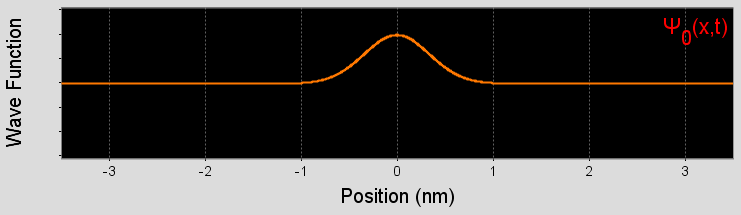
\includegraphics[width=5in]{Ground_Wave.png}
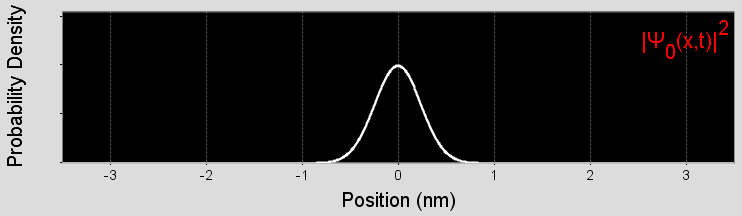
\includegraphics[width=5in]{Ground_Probability.png}
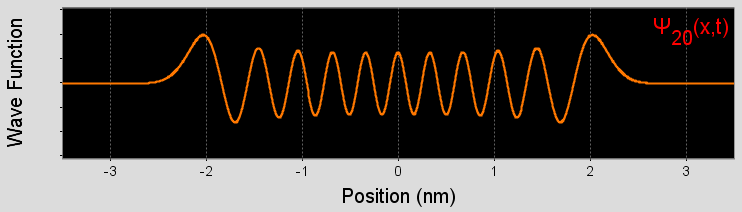
\includegraphics[width=5in]{20_Wave.png}
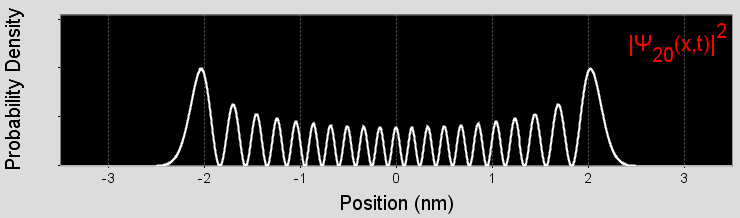
\includegraphics[width=5in]{20_Probability.png}
\end{figure}
I have read through all the side bar links and understand them.
\end{document}
